\section{Evaluation framework - DocTide Labs}
\label{sec:DocTideLabs}
A long side the development of the LLM-based autonomous agent DocTide, this paper also proposes a framework, for conducting \textit{'objective evaluation'}\cite{wang2024survey} of said agents behavior and performance. Moving forward, this framework will be referred to as DocTide Labs.

DocTide Labs is an implementation of a \textit{'real world simulation protocol'}, in which the goal is to simulate an immersive environment where in the agent autonomously can complete tasks while chosen metrics\footnote{For the scope of this paper the only metrics collected are 'semantic similarity' and 'success rate', but the implemented evaluation protocol allows to be reused for collection of further metrics, if these where to be implemented.} are measured and collected\cite{wang2024survey}.
\\ \\
DocTide is developed as a prototype to automate the task of making function-level documentation within the environment of a Github repository, which is why DocTide Labs is developed to simulate exactly that. By replaying the commit history of a chosen Github repository and removing human generated documentation, DocTide Labs simulates the environment in which the agent is developed to run.

\subsection{Functionality\textcolor{red}{(Design?)} of DocTide Labs}
The logic and functionality of DocTide Labs is explained in the following sections. For a visualization of the entire flow of state when running an evaluation, see Figure \ref{fig:flow_labs}.
\\ \\
The only prerequisites to run DocTide Labs is a repository that you want to simulate in the evaluation, together with a Github Personal Access Token with `admin:org, gist, repo, workflow' permissions of said repository.

Furthermore before running, the part of the commit history to simulate during the evaluation is also specified.

\begin{figure}[H]
\centering
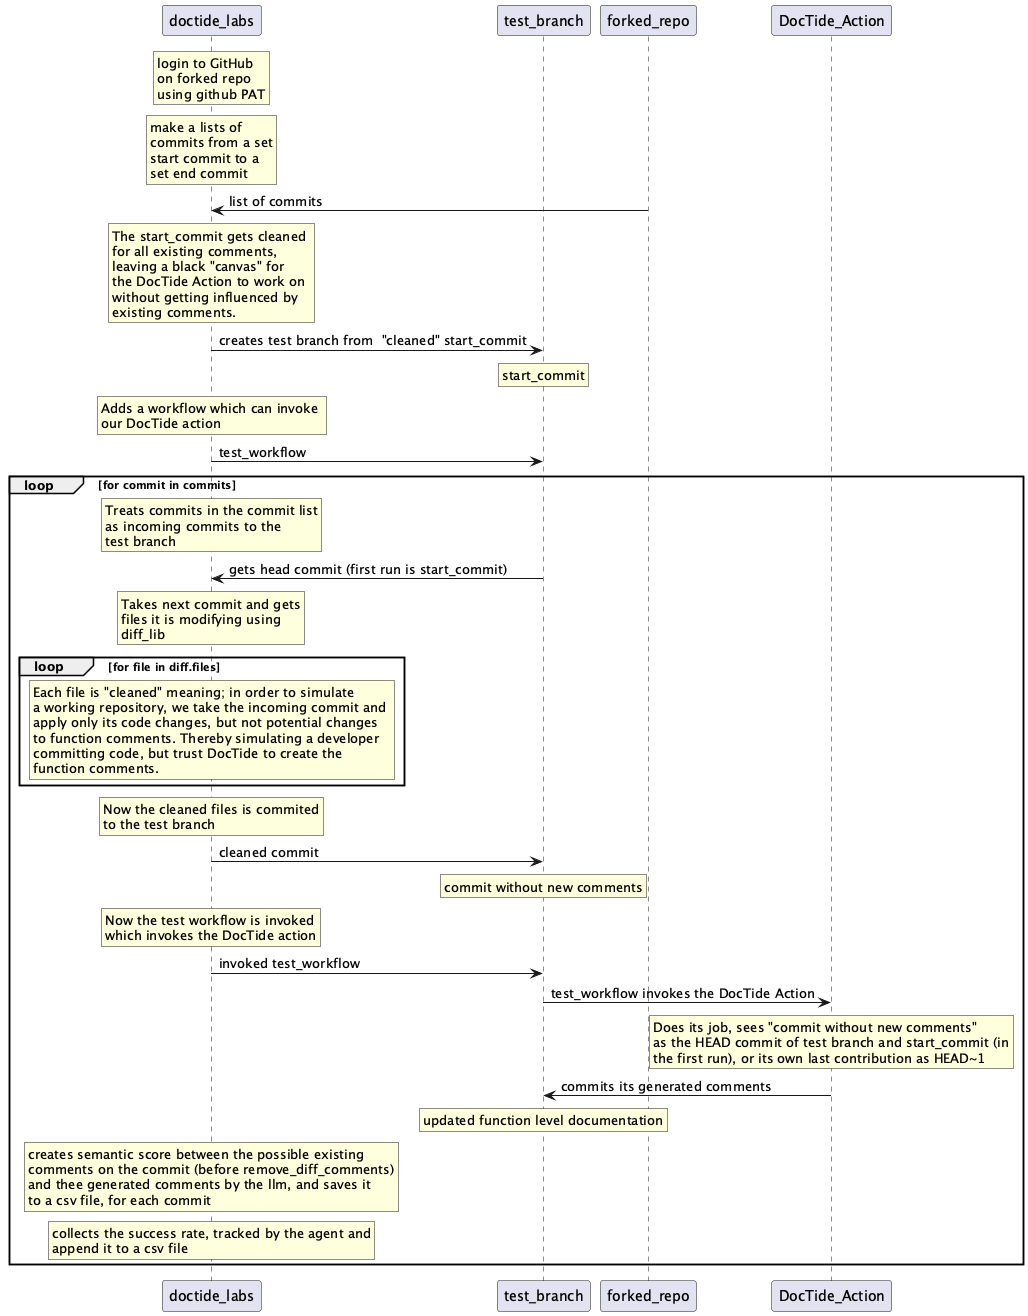
\includegraphics[width=0.7\linewidth]{Figures/doctide_labs_flow_chart.png}
\caption{The flow of the state the evaluation setup, shows how commits are collected from a repository, preprocessed, and then committed to the test-branch, where DocTide is invoked, and finally metrics are collected}
\label{fig:flow_labs}
\end{figure}

\subsubsection{Data Collection and setup}
The first step in DocTide Labs is to collect a 'dataset' of commits to use in the evaluation, which is done by fetching the specified commits from the chosen repository. All python files are cleaned from existing documentation, and a Test Branch is then created by checking out the oldest of the fetched commits, making this a 'snapshot copy' of the chosen repository in a previous time in history, but without the history of documenation.

Finally a workflow utilizing the DocTide Action is manually added to the repository, enabling DocTide Labs to trigger this later in the evaluation.

\subsubsection{Commit processing}
Next DocTide Labs then iterates through the fetched commits, processing each of them sequentially. In each iteration, first a diff between the commit and the head of the test branch is calculated, which serves to identify the files modified in the commit at hand. In order to best simulate the environment and conditions for which the agent is developed, each file in from the commit is then 'cleaned from comments'. This 'cleaning step' utilizes Tree-sitter\footnote{\url{https://tree-sitter.github.io/tree-sitter/}} to identify and remove all function-level documentation in the file, leaving only the code changes introduced with the commit. The diff of the cleaned file, and the head of the test branch is used to restore any documentation introduced by the agent in previous iterations.

Each 'cleaned commit' is then committed to the test branch, and the workflow utilizing the DocTide Action is triggered. This finalizes the simulation of the agent running continuously on a live repository that evolves over time.

\subsubsection{Agent execution and metric collection}
When triggered the workflow runs the agent, which generates the documentation based on the new commit. The Doctide Action is run with the 'testing' flag set to true, which allows it to directly merge in its generated documentation, enabling the continuous running of multiple iterations, without human intervention during the evaluation. 

Further more this enables the collection of metrics, which upon end of evaluation is returned in two csv files.
